\documentclass[a4paper,11pt]{article}

\usepackage[pdftex]{graphicx}
%\usepackage{babel}
\usepackage[utf8]{inputenc}
\usepackage[T1]{fontenc}
%\usepackage[T1,mtbold,lucidacal,mtplusscr,subscriptcorrection]{mathtime}
\usepackage{times}
\usepackage{amsmath}
\usepackage{url}
\usepackage{enumerate}
\usepackage{parskip}
\usepackage[colorlinks,urlcolor=black]{hyperref}
\usepackage{microtype}

% if not draft, the smaller printable area makes the paper more readable
\topmargin -4mm
\oddsidemargin 0mm
\textheight 225mm
\textwidth 150mm

\usepackage{xcolor}
\hypersetup{
    colorlinks,
    linkcolor={red!50!black},
    citecolor={blue!50!black},
    urlcolor={blue!80!black}
}


%\parskip=\baselineskip

\DeclareMathOperator{\E}{E}
\DeclareMathOperator{\Var}{Var}
\DeclareMathOperator{\var}{var}
\DeclareMathOperator{\Sd}{Sd}
\DeclareMathOperator{\sd}{sd}
\DeclareMathOperator{\Bin}{Bin}
\DeclareMathOperator{\Beta}{Beta}
\DeclareMathOperator{\Poisson}{Poisson}
\DeclareMathOperator{\betacdf}{betacdf}
\DeclareMathOperator{\Invchi2}{Inv-\chi^2}
\DeclareMathOperator{\logit}{logit}
\DeclareMathOperator{\N}{N}
\DeclareMathOperator{\U}{U}
\DeclareMathOperator{\tr}{tr}
\DeclareMathOperator{\trace}{trace}

% Parenthesis \left  \right -fix
\renewcommand*{\l}{\mathopen{}\mathclose\bgroup\left}
\renewcommand*{\r}{\aftergroup\egroup\right}


% Horizontal line
\newcommand{\HRule}{\rule{\linewidth}{0.5mm}}

% \pagestyle{empty}


% Stan source code block
\usepackage{listings}


\usepackage{Sweave}
\begin{document}
\input{ex7-concordance}
% \thispagestyle{empty}

\section*{Bayesian data analysis -- Assignment 7}


\subsubsection*{General information}

\begin{itemize}
\itemsep0em 
\item The recommended tool in this course is R (with the IDE R-Studio). You can download R \href{https://cran.r-project.org/}{\textbf{here}} and R-Studio \href{https://www.rstudio.com/products/rstudio/download/}{\textbf{here}}. There are tons of tutorials, videos and introductions to R and R-Studio online. You can find some initial hints \href{https://www.rstudio.com/online-learning/}{\textbf{here}}. 
\item  You can write the report with your preferred software, but the outline of the report should follow the instruction in the R markdown template that can be found \href{https://raw.githubusercontent.com/avehtari/BDA_course_Aalto/master/templates/assignment_template.rmd}{\textbf{here}}. 
\item  Report all results in a single, {\bf anonymous} *.pdf -file and return it to \href{peergrade.io}{\textbf{peergrade.io}}. 
\item Many of the exercises can be checked using the R package \texttt{markmyassignment}. Information on how to install and use the package can be found \href{https://cran.r-project.org/web/packages/markmyassignment/vignettes/markmyassignment.html}{\textbf{here}}.
\item The course has its own R package with data and functionality to simplify coding. To install the package just run the following:
\begin{enumerate}
\item \texttt{install.packages("devtools")}
\item \texttt{devtools::install\_github("avehtari/BDA\_course\_Aalto", \\ subdir = "rpackage")}
\end{enumerate}
\item Many of the exercises can be checked automatically using the R package \\ \texttt{markmyassignment}. Information on how to install and use the package can be found \href{https://cran.r-project.org/web/packages/markmyassignment/vignettes/markmyassignment.html}{\textbf{here}}.
\item Additional self study exercises and solutions for each chapter in BDA3 can be found \href{http://www.stat.columbia.edu/~gelman/book/solutions3.pdf}{\textbf{here}}.
\item If you have any suggestions or improvements to the course material, please feel free to create an issue or submit a pull request to the public repository!!
\end{itemize}

\newpage

\subsubsection*{Information on this assignment}
This exercise is related to Chapter 5. The maximum amount of points from this assignment is 6. 

\textbf{Reading instructions:} Chapter 5 in BDA3, see \href{https://github.com/avehtari/BDA_course_Aalto/blob/master/chapter_notes/BDA_notes_ch5.pdf}{\textbf{here}}.

\textbf{Grading instructions:} The grading will be done in peergrade. All grading questions and evaluations for assignment 7 can be found \href{https://github.com/avehtari/BDA_course_Aalto/blob/master/exercises/ex7_rubric.md}{\textbf{here}}

\textbf{Reporting accuracy:} As many significant digits as justified by the Monte Carlo error and posterior accuracy.

\textbf{Installing and using {\tt rstan}:} See the Stan demos on how to use Stan from R. The university Ubuntu desktops have the necessary libraries installed so there should be no need to install anything. To install Stan on your laptop, see the instructions below.

In R, install package {\tt rstan}. Installation instructions on Linux, Mac and Windows can be found at \url{https://github.com/stan-dev/rstan/wiki/RStan-Getting-Started}. Additional useful packages are {\tt loo}, {\tt bayesplot} and {\tt shinystan} (but you don't need these in this exercise). For Python users, the {\tt Arviz} library may be relevant. 

Stan manual can be found at \url{http://mc-stan.org/documentation/}. From this website, you can also find a lot of other useful material about Stan. 

\newpage


\subsection*{1. Linear model: drowning data with Stan (3p)}

The provided data {\tt drowning} in the {\tt aaltobda} package contains the number of people drown per year in Finland 1980--2016.
%
We are going to fit a linear model with Gaussian noise to these data using time as the predictor and number of drownings as the target variable (see the related linear model example for the Kilpisjärvi-temperature data in the example Stan codes).
We have two objective questions:
\begin{itemize}
    \item [i)] What is the trend of the number of people drown per year? We would plot the histogram of the slope of the linear model.
    \item [ii)] What is the prediction for the year 2019? We would plot the histogram of the posterior predictive distribution for the number of people drowning at $\tilde x=2019$.
\end{itemize}

To access the data, use:

\begin{Schunk}
\begin{Sinput}
> library(aaltobda)
> data("drowning")
\end{Sinput}
\end{Schunk}


\begin{enumerate}

\item The provided Stan code in Listing~\ref{listing1} is almost correct for the given problem. However, there are two crucial mistakes. Find these two mistakes and fix them. Report the original mistakes and your fixes clearly in your report. Include the \emph{full} Stan code in your report.

\item The provided broken code does not define any prior for the parameters. In Stan, this corresponds to using a uniform prior. In addition to the two fixes discussed above, we would like to apply a weakly-informative prior $\operatorname{N}(0, \tau^2)$ for the slope parameter {\tt beta} into the code. It is very unlikely that the mean number of drownings changes more than 50 \% in one year. The approximate historical mean yearly number of drownings is 138. Hence, set $\tau$ so that the following holds for the prior probability for {\tt beta}: $\operatorname{Pr}(-69 < \text{{\tt beta}} < 69) = 0.99$. Determine suitable value for $\tau$ and report the approximate numerical value for it in the report. 
\item Using the obtained $\tau$, implement the desired prior in the Stan code. In the report, in a separate section, indicate clearly how you carried out your prior implementation, e.g.\ ``Added line \dots in block \dots''.

\textbf{Hint!} Example resulting plots for the problem, with the fixes and the desired prior applied, are shown in Figure~\ref{fig1}. If you want, you can use these plots as a reference for testing if your modified Stan code produces similar results. However, running the inference and comparing the plots is not required. 
\end{enumerate}


\begin{lstlisting}[
    float,
    caption=Broken Stan code for question 1,
    label=listing1,
    basicstyle=\footnotesize\ttfamily,
    numbers=left,
    xleftmargin=2.7em,
    frame=single,
    framexleftmargin=2.2em
]
data {
    int<lower=0> N;  // number of data points
    vector[N] x;     // observation year
    vector[N] y;     // observation number of drowned
    real xpred;      // prediction year
}
parameters {
    real alpha;
    real beta;
    real<upper=0> sigma;
}
transformed parameters {
    vector[N] mu;
    mu = alpha + beta*x;
}
model {
    y ~ normal(mu, sigma);
}
generated quantities {
    real ypred;
    ypred = normal_rng(mu, sigma);
}
\end{lstlisting}

\begin{figure}[htb]
\centering
   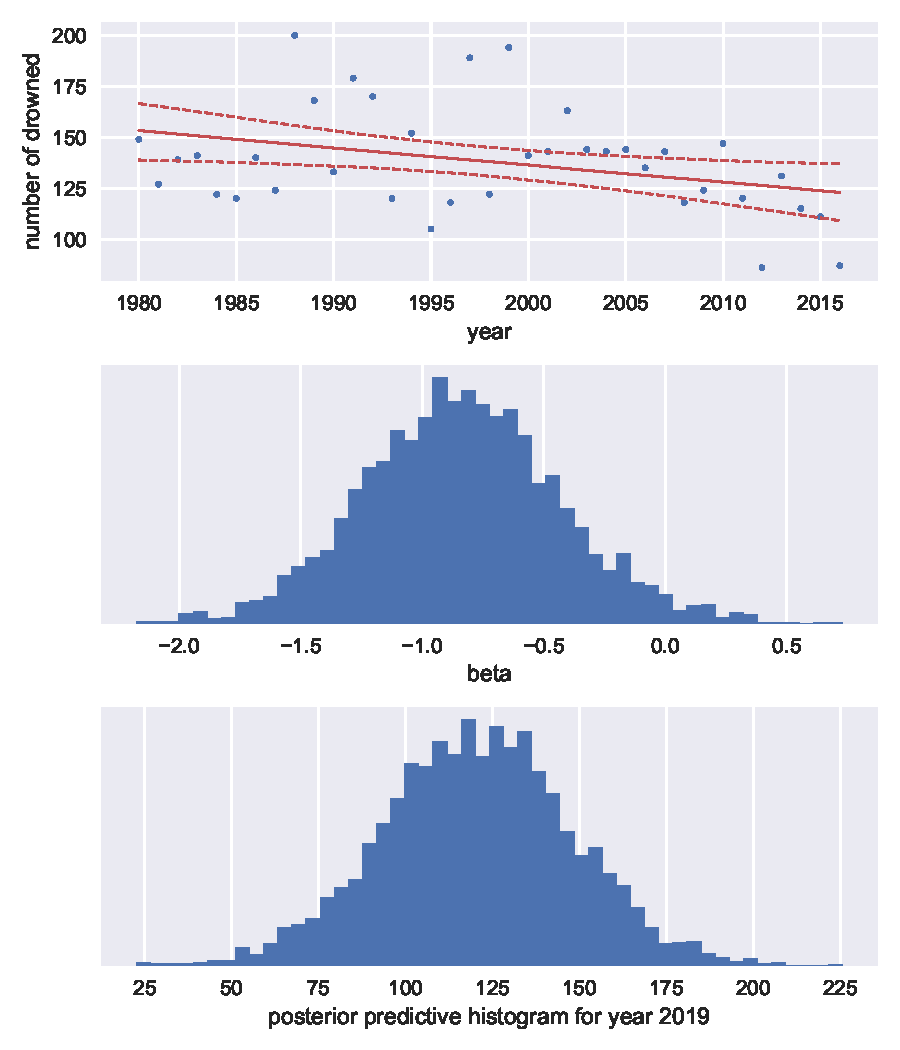
\includegraphics[width=0.56\textwidth]{ex7_fig1.pdf}
\caption{Example plots for the results obtained for problem in the question 1. In the first subplot, the red lines indicate the resulting 5 \%, 50 \%, and 95 \% posterior quantiles for the transformed parameter {\tt mu} at each year.}\label{fig1}
\end{figure}


\newpage

\subsection*{2. Hierarchical model: factory data with Stan (3p)}

The {\tt factory} data in the {\tt aaltobda} package contains quality control measurements from 6 machines in a factory (units of the measurements are irrelevant here). In the data file, each column contains the measurements for a single machine. Quality control measurements are expensive and time-consuming, so only 5 measurements were done for each machine. In addition to the existing machines, we are interested in the quality of another machine (the seventh machine). To read in the data, just use:

\begin{Schunk}
\begin{Sinput}
> library(aaltobda)
> data("factory")
\end{Sinput}
\end{Schunk}

Implement a separate, pooled and hierarchical Gaussian model described in Section 11.6 using Stan. In the pooled model, all the measurements are combined and no distinction is made between the machines. In the separate model, each machine has its model. Similarly, as in the model described in the book, use the same measurement standard deviation $\sigma$ for all the groups in the hierarchical model. In the separate model, however, use separate measurement standard deviation $\sigma_j$ for each group $j$. Use Stan's default uniform prior for all (non-hiearchical) parameters.


Using each of the three models -- separate, pooled, and hierarchical -- report (comment and, if applicable, plot histogram):
\begin{itemize}
    \item [i)] the posterior distribution of the mean of the quality measurements of the sixth machine
    \item [ii)] the predictive distribution for another quality measurement of the sixth machine
    \item [iii)] the posterior distribution of the mean of the quality measurements of the seventh machine.
\end{itemize}


\textbf{Hint!} See the example Stan-codes \href{http://avehtari.github.io/BDA_R_demos/demos_rstan/rstan_demo.html#8_comparison_of_k_groups_with_hierarchical_models}{\textbf{here}} for the comparison of $k$ groups with and without the hierarchical structure. What you need to do is change the dataset, implement the prediction for the future measurement of the sixth machine, and figure out the distribution for the mean of the quality measurements for the seventh machine in the hierarchical model.


\end{document}

%%% Local Variables:
%%% mode: latex
%%% TeX-master: t
%%% End:
